\chapter{Характеристика объекта исследования}
\section{Характеристика грунтового массива исследуемого участка}
Анализ проводился на образцах, отобранных на участке исследования  под жилой комплекс Саларьево-парк.

Условия залегания, распространения, состав, состояние  грунтов зависят от возраста и~генезиса и~создают довольно разнородную картину. Изучались дисперсные грунты, представленные глинами и~суглинками твердой, полутвердой и~тугопластичной консистенции.


Геологический разрез на участке представлен разновозрастными отложениями различного генезиса.
Геологический разрез исследуемой территории был изучен на глубину 29,0~м, и~представлен следующими стратиграфическими подразделениями:

 Среднечетвертичные ледниковые отложения московского горизонта \q{g}{II}{ms} залегают под флювиогляциальными отложениями.
 Они представлены суглинками от коричневых до красновато-коричневых, тугопластичными, местами полутвердыми, песчанистыми, с~прослоями супеси и~песка, с~включениями дресвы и~щебня преимущественно карбонатных пород до 10"---15~\%.
 В~подошве с~прослоями песка мелкого коричневого, насыщенного водой.
 Их мощность колеблется от 0,9 м до 2,1 м с~абс. отм. подошвы 179,6"---180,3~м.
 Этот слой ИГЭ-6 (Технический отчет. Саларьево-парк,~2019) \cite{moshkin2019}.

Нижне-среднечетвертичные флювиогляциальные, ледниково-озерные, аллювиальные и~озерные отложения донского-московского горизонта \q{f,lg}{I-II}{ds-ms} залегают повсеместно под флювиогляциальными и~ледниковыми отложениями московского горизонта. 
Они представлены суглинками в~кровле и~в~подошве, и~глинами в~средней части. Суглинки тугопластичные от светло-коричневых до зеленовато-коричнево-серых, тугопластичные, местами до полутвердых, песчанистые, слабо слоистые, с~редкими включениями гравия и~гальки, залегают преимущественно в~кровле и~подошве флювиогляциальных отложений. 
Мощность суглинков колеблется от 1,1 до 3,4~м. 
Глины серые, темно-серые, с~зеленоватым оттенком, полутвердые, в~кровле 0,2~м тугопластичные, слоистые, пылеватые, с~единичными включениями гравия и~гальки, преимущественно залегают в~средней части толщи флювиогляциальных отложений, и~вскрыты всеми скважинами. 
Мощность глин составила 2,8"---3,8 м. 
Общая мощность флювиогляциальных отложений донского-московского горизонта составляет 6,7"---8,2~м с~абсолютной отметкой подошвы 171,6"---173,4~м. 
Суглинки тугопластичные "--- ИГЭ-7, глины полутвердые "--- ИГЭ-8 (Технический отчет. Саларьево-парк,~2019).

Ниже залегают нижнечетвертичные ледниковые отложения донского горизонта \q{g}{I}{ds}. 
Они представлены мощной толщей суглинков коричневых, до темно-серо-коричневых, полутвердых, в~кровле 0,1"---0,3 м тугопластичных, песчанистых, с~включениями дресвы и~щебня преимущественно карбонатных пород до 15\%. 
Мощность этих суглинков составила 14,4 м, с~абсолютной отметкой подошвы 157,2~м. 
Слой образует ИГЭ-9 (Технический отчет. Саларьево-парк,~2019) \cite{moshkin2019}.

Химический состав воды характеризуется как сульфатно-хлоридно-гидрокарбонатный магниево-кальциевый пресный с~минерализацией 0,9~г/л, рН~равен~7,9. 
Вода неагрессивная к~бетону на портландцементе любых марок, слабоагрессивная к~железобетонным конструкциям. 
Отмечается средняя коррозионная агрессивность к~свинцовым и~высокая к~алюминиевым оболочкам кабелей (Технический отчет. Саларьево-парк,~2019) \cite{moshkin2019}.


Для испытаний были выбраны образцы четырёх разновидностей: 
суглинки тугопластичные московского горизонта (ИГЭ-6), 
суглинки тугопластичные московско-донского горизонта (ИГЭ-7), 
суглинки полутвердые московско-донского горизонта (ИГЭ-8), 
ледниковые отложения донского горизонта (ИГЭ-9). 




 \section{Минералогический состав грунтов} 

В целях дополнительного изучения образцов был сделан рентгено-структурный анализ 
ледниковых и~озерно-ледниковых отложений московского и~донского горизонта 
в~лаборатории кафедры инженерной и~экологической геологии 
геологического факультета Московского государственного университета им.~М.\:В.\:Ломоносова 
аналитиками инж. 1~кат. С./:А./:Гараниной и~вед.~инж. С.\:В.\:Закусиным, ст.\:н.\:с. В.\:В.\:Крупской.


Результаты исследований минерального состава грунтов представлены в~таблице \ref{tab:mineral}, 
где \texttt{GJ6874} "---суглинок тугопластичный (ИГЭ-7), 
\texttt{GJ6890} "--- глина полутвердая (ИГЭ-8а), 
\texttt{GJ6835} "--- суглинок тугопластичный (ИГЭ-6), 
\texttt{GJ6864} "--- глина полутвердая (ИГЭ-9).


\begin{table}[]
    \centering
    \small
    \caption{Минеральный состав образцов (вес. \%)} \label{tab:mineral}
    \begin{tabular}{@{}lrrrr@{}}
    \toprule
    Минерал & \texttt{GJ6874} &	\texttt{GJ6890} & \texttt{GJ6835} & \texttt{GJ6864}  \\ \midrule
    Смектит*	& 21.5	& 27.0	& 9.0	& 18.6 \\
    Хлорит	& 1.5	& 0.0	& 2.0	& 2.8 \\
    Иллит	& 10.2	& 6.0	& 8.3	& 4.9 \\
    Каолинит	& 4.6	& 4.6	& 1.4	& 3.5 \\
    Кварц	& 43.1	& 51.2	& 41.6	& 45.2 \\
    Плагиоклазы (Альбит)	& 8.1	& 4.6	& 17.0	& 3.8 \\
    КПШ (Микроклин)	& 10.2	& 5.7	& 10.3	& 5.6 \\
    Кальцит	& 0.0	& 0.0	& 4.4	& 6.4 \\
    Сидерит	& 0.4	& 0.0	& 0.3	& 0.0 \\
    Доломит	& 0.4	& 0.0	& 3.6	& 9.2 \\
    Анкерит	& 0.0	& 0.9	& 0.0	& 0.0 \\
    Роговая обманка	& 0.0	& 0.0	& 2.1	& 0.0 \\ \bottomrule
    \end{tabular}
    \\ 
    \raggedright 
    *Вероятно присутствие смешанослойного минерала иллит-смектит с~преобладанием смектитовых (набухающих) пакетов. Для точной диагностики требуется выделение глинистой фракции.
\end{table}
	
По результатам минералогического анализа грунта можно сказать о типе ассоциации минералов. 
Исходя из значений в~таблице \ref{tab:mineral}, приведенной выше, состав исследуемых образцов можно причислить к~типу ассоциации 1а (Шлыков, 2006) \cite{Sh_2006}.


\section{Гранулометрический состав грунтов}

Были проведены определения гранулометрического состава озерно-ледниковых и~ледниковых отложений московского и~донского горизонтов ареометрическим методом. Определение проводилось по ГОСТ 12536-2014. В~результате построена треугольная диаграмма гранулометрического состава (рис. \ref{Fig:Ferre}).

Гранулометрический состав определялся только для песчанисто-глинистых фракций, без учета крупнообломочной составляющей.
По результатам гранулометрического состава были построены кумулятивные кривые (рис. \ref{fig:curves}).
Кривые построены в~полулогарифическом масштабе, 
по оси абсцисс отложены логарифмы диаметров частиц, 
а по оси ординат накопленное содержание фракции в~процентах.

{
\small
\pgfplotsset{
%samples=15,
width=0.45\linewidth,
xlabel={Диаметр частиц $d$, мм},
ylabel={Содержание частиц, \%},
%extra y ticks={45},
legend pos=north west,
ymin = 0,
ymax = 100,
}

\begin{figure}
	{\centering
	\small
	\subbottom[ИГЭ-6]{
\begin{tikzpicture}
    \begin{semilogxaxis}[]
    
    % ИГЭ-6
    \addplot[smooth, no marks, red!70!orange!80!black] table [x=Size, y=GJ6805, col sep=semicolon] {data/hydrometer-cumulative.csv};
    \addplot[smooth, no marks, red!70!orange!80!black] table [x=Size, y=GJ6807, col sep=semicolon] {data/hydrometer-cumulative.csv};
    \addplot[smooth, no marks, red!70!orange!80!black] table [x=Size, y=GJ6838, col sep=semicolon] {data/hydrometer-cumulative.csv};
    \addplot[smooth, no marks, red!70!orange!80!black] table [x=Size, y=GJ6835, col sep=semicolon] {data/hydrometer-cumulative.csv};
    
    \end{semilogxaxis}
\end{tikzpicture}}
	\hfill
	\subbottom[ИГЭ-7]{\begin{tikzpicture}
    \begin{semilogxaxis}[]
    
    % ИГЭ-7
    \addplot[smooth, no marks, lime!40!black] table [x=Size, y=GJ6898, col sep=semicolon] {data/hydrometer-cumulative.csv};
    \addplot[smooth, no marks, lime!40!black] table [x=Size, y=GJ6874, col sep=semicolon] {data/hydrometer-cumulative.csv};
    
    \end{semilogxaxis}
\end{tikzpicture}}
	}
	\\
	{\centering
	\small
	\subbottom[ИГЭ-8]{\begin{tikzpicture}
    \begin{semilogxaxis}[]
    
    % ИГЭ-8
    \addplot[smooth, no marks, green!10!lime!30!black] table [x=Size, y=GJ6822, col sep=semicolon] {data/hydrometer-cumulative.csv};
    \addplot[smooth, no marks, green!10!lime!30!black] table [x=Size, y=GJ6884, col sep=semicolon] {data/hydrometer-cumulative.csv};
    \addplot[smooth, no marks, green!10!lime!30!black] table [x=Size, y=GJ6846, col sep=semicolon] {data/hydrometer-cumulative.csv};
    \addplot[smooth, no marks, green!10!lime!30!black] table [x=Size, y=GJ6890, col sep=semicolon] {data/hydrometer-cumulative.csv};
    \addplot[smooth, no marks, green!10!lime!30!black] table [x=Size, y=GJ6888, col sep=semicolon] {data/hydrometer-cumulative.csv};
    
    
    \end{semilogxaxis}
\end{tikzpicture}}
	\hfill
	\subbottom[ИГЭ-9]{
\begin{tikzpicture}
    \begin{semilogxaxis}[]
    
    % ИГЭ-9
    \addplot[smooth, no marks, red!80!orange!50!black] table [x=Size, y=GJ6865, col sep=semicolon] {data/hydrometer-cumulative.csv};
    \addplot[smooth, no marks, red!80!orange!50!black] table [x=Size, y=GJ68A3, col sep=semicolon] {data/hydrometer-cumulative.csv};
    \addplot[smooth, no marks, red!80!orange!50!black] table [x=Size, y=GJ68B7, col sep=semicolon] {data/hydrometer-cumulative.csv};
    \addplot[smooth, no marks, red!80!orange!50!black] table [x=Size, y=GJ68A0, col sep=semicolon] {data/hydrometer-cumulative.csv};
    
    \end{semilogxaxis}
\end{tikzpicture}}
	}

	\caption{Кумулятивные кривые гранулометрического состава исследованных грунтов}
	\label{fig:curves}
\end{figure}

}

При сопоставление результатов гранулометрического и~минералогического анализа было замечено, 
что содержание песчаных фракция примерно соотвествует содержанию кварца, пылеватых фракций примерно соответсвует плагиоклазов и калиевых полевых шпатов, а содержание глинистой фракции примерно соответсвует содержанию смектита, хлорита, иллита, каолинита и других глинистых минералов.
Такая взаимосвязь дисперсности и минерального состава вовсе не случайна. Это объясняется тем, что размер частиц обусловен процессами литогенеза, в результате которого частицы дробятся и претерпевают изменение минералов (Грунтоведение, 2005)\cite{grunt2005}.

Треугольная диаграмма является удобным способом показать большое число результатов и~выявить характерные области.

На рисунке \ref{Fig:Ferre} видно, что моренные отложения московского и~донского горизонтов образуют довольно кучную группу в~области песчанистых суглинков.
Отложения различного генезиса московско-донского горизонта, напротив, более разнообразны по составу, но тяготеют к~области 
пылеватых суглинков.

\begin{figure}[ht]
    \centering
    \small
    %\pgfplotstableset{format=file}
\pgfplotsset{width=0.7\linewidth}

\begin{tikzpicture}
    \begin{ternaryaxis}[
        legend cell align={left},
        %title=Spinel,
        ternary limits relative=false,
        %width=10cm,
        %height=10cm,
        xmax=100,
        ymax=100,
        zmax=100,
        minor tick num=1,
        grid=both,
        xlabel={Глина, \%},
        xlabel style={
            at={(axis cs:100,0,0)},
            anchor=south,
            yshift=16pt,
            align=center
        },
        ylabel={Песок, \%},
        ylabel style={
            at={(axis cs:0,100,0)},
            anchor=10,
            xshift=-11pt,
            yshift=-16pt,
            align=center
        },
        zlabel={Пыль, \%},
        zlabel style={
            at={(axis cs:0,0,100)},
            anchor=north west,
            xshift=16pt,
            yshift=-11pt,
            align=center
        },
    ]

        \addplot3 [only marks, mark=*, red!70!orange!80!black] 
        table [x=Clay, y=Sand, z=Silt, col sep=semicolon, row sep=newline] {data/gran-activity-6.csv};
        \addlegendentry{ИГЭ-6}

        \addplot3 [only marks, mark=*, lime!50!yellow!40!black]
        table [x=Clay, y=Sand, z=Silt, col sep=semicolon, row sep=newline] {data/gran-activity-7.csv};
        \addlegendentry{ИГЭ-7}

        \addplot3 [only marks, mark=*, green!50!lime!30!black] 
        table [x=Clay, y=Sand, z=Silt, col sep=semicolon, row sep=newline] {data/gran-activity-8.csv};
        \addlegendentry{ИГЭ-8}

        \addplot3+[only marks, mark=*, red!80!orange!50!black] 
        table [x=Clay, y=Sand, z=Silt, col sep=semicolon, row sep=newline] {data/gran-activity-9.csv};
        \addlegendentry{ИГЭ-9}

    \end{ternaryaxis}
\end{tikzpicture}
    \caption{Треугольная диаграмма Ферре для выражения гранулометрического состава исследованных грунтов}
    \label{Fig:Ferre}
\end{figure}

Треугольная диаграмма служит отправной точкой для некоторых классификаций грунтов, например по В.\;В. Охотину (таблица \ref{tab:oxot}).

\begin{table}[ht]
    \centering
    %\small
    \caption{Классификация грунтов по Охотину В.\:В.} \label{tab:oxot}
    %\renewcommand*{\arraystretch}{1.2}
    \begin{tabular}{cl}
    %\toprule
    %ИГЭ & Разновидности грунта \\
    %\midrule
    ИГЭ-6 \dotfill &  от супеси тяжелой до суглинка легкого \\
    ИГЭ-7 \dotfill &  от суглинка среднего пылеватого до тяжелого пылеватого \\
    ИГЭ-8 \dotfill &  от суглинка легкого до тяжелого пылеватого \\
    ИГЭ-9 \dotfill &  от суглинка легкого до среднего \\
    %\bottomrule
    \end{tabular}
    %\\ 
\end{table}

Классификация исследованных грунтов по гранулометрическому составу согласно ГОСТ 25100-2011 приведена в приложении \ref{app:tp}.

 
\section{Химические состав грунтов}

Химический анализ водных вытяжек позволяет определить состав растоворимых в~воде минералов грунтов.
Анализ проводился методом капиллярного элетрофореза. 

Результаты представлены в~таблице \ref{tab:chem}.

\begin{table}[]
    \centering
    \tiny
    \caption{Химических состав водных вытяжек грунтов} \label{tab:chem}
    \begin{tabular}{@{}lrrrrrrrrrrrrr@{}}
    \toprule
    Образец & pH & NH$_4^+$ &	K$^+$ & Na$^+$ & Mg$^{2+}$ & Ca$^{2+}$ &	Сl$^-$ &	NO$_2^-$	   & SO$_4^{3-}$ &	NO$_3^-$ &	Fe$^{2+,3+}$ &	HCO$_3^-$   & УЭП \\ \midrule
    \texttt{GJ68A0} & 7,22 & н п о & 1,81 & 1,71 & 1,21 &  5,93 & 1,58 & н п о &  1,99 & 3,59 & 0,15 & 23,64 &  43,7 \\
    \texttt{GJ68A3} & 7,70 & 0,16  & 3,35 & 2,26 & 2,97 & 16,49 & 1,97 & н п о &  1,53 & 5,64 & 0,18 & 67,25 & 108,1 \\
    \texttt{GJ68B7} & 7,51 & н п о & 6,92 & 1,66 & 7,33 & 43,88 & 0,68 & н п о & 111,6 & 0,82 & 0,22 & 40,57 & 288,0 \\
    \texttt{GJ6805} & 7,67 & н п о & 1,86 & 2,42 & 2,73 & 16,29 & 3,32 & н п о &  4,69 & 3,99 & 0,17 & 56,88 & 101,9 \\
    \texttt{GJ6807} & 7,72 & 0,18  & 2,11 & 2,28 & 2,55 & 14,18 & 0,97 & н п о &  1,17 & 5,78 & 0,13 & 60,70 & 102,7 \\
    \texttt{GJ6822} & 7,26 & н п о & 1,71 & 3,27 & 1,85 &  7,27 & 3,05 & н п о &  5,71 & 0,56 & 0,16 & 31,72 &  70,1 \\
    \texttt{GJ6835} & 7,39 & н п о & 0,85 & 1,66 & 2,12 & 11,77 & 0,95 & н п о &  3,59 & 3,59 & 0,19 & 41,79 &  81,6 \\
    \texttt{GJ6838} & 7,23 & н п о & 0,79 & 1,63 & 2,46 & 13,30 & 1,03 & н п о &  2,57 & 4,63 & 0,25 & 50,33 &  87,0 \\
    \texttt{GJ6846} & 7,73 & 0,13  & 1,27 & 2,60 & 2,03 & 10,25 & 2,97 & н п о &  5,51 & 0,87 & 0,15 & 39,19 &  72,2 \\
    \texttt{GJ6855} & 7,63 & н п о & 2,38 & 2,37 & 2,73 & 14,28 & 1,98 & н п о &  2,50 & 4,36 & 0,18 & 56,43 & 100,9 \\
    \texttt{GJ6864} & 7,08 & н п о & 3,52 & 1,79 & 3,11 & 16,01 & 1,87 & н п о &  4,17 & 0,29 & 0,12 & 67,41 & 107,1 \\
    \texttt{GJ6865} & 7,30 & н п о & 1,36 & 3,04 & 1,76 &  9,35 & 1,14 & н п о &  6,17 & 0,54 & 0,10 & 39,65 &  75,6 \\
    \texttt{GJ6874} & 7,16 & 0,50  & 1,38 & 3,00 & 4,62 & 22,71 & 6,11 & н п о & 41,93 & 0,59 & 0,13 & 39,04 & 154,1 \\
    \texttt{GJ6884} & 7,37 & н п о & 3,12 & 4,02 & 2,31 & 11,39 & 3,15 & н п о &  3,53 & 5,39 & 0,22 & 50,33 &  73,5 \\
    \texttt{GJ6888} & 7,23 & 0,28  & 0,65 & 2,83 & 2,48 & 12,28 & 0,99 & 0,185 &  1,93 & 6,76 & 0,28 & 51,85 &  65,3 \\
    \texttt{GJ6890} & 7,19 & 0,20  & 0,61 & 2,28 & 2,23 & 10,48 & 0,69 & н п о &  1,97 & 0,89 & 0,19 & 45,75 &  68,7 \\
    \texttt{GJ6898} & 6,95 & н п о & 0,59 & 2,27 & 1,70 &  7,82 & 2,06 & н п о &  3,08 & 7,12 & 0,14 & 27,45 &  63,3 \\
    \bottomrule 
    \end{tabular}
    \\ 
\end{table}

Электрофореграммы представлены в~Приложении \ref{app:kapel}

%По степени засоленности все испытанные грунты относятся к~группе незасоленных грунтов.

\section{Физические свойства грунтов}

Испытания грунтов проводились в~соответствии с~методами, приведенными в~действующих нормативных документах:
плотность $\rho$, 
плотность твердых частиц $\rho_s$, 
влажность $w_e$, 
влажность на границе раскатывания и~текучести ($w_L$ и~$w_p$) "--- по ГОСТ 5180-2015. 
Рассчитаны такие параметры для глинистых грунтов, как
плотность сухого грунта $\rho_d$,  
коэффициент водонасыщения $S_r$, 
число пластичности $I_p$ 
и показатель текучести $I_L$ по ГОСТ 25100-2011.
Результаты лабораторного определения физических свойств приведены в~Приложении \ref{app:tp}.



Физические свойства, химический и~гранулометрический состав были определены в~Центральной грунтово-химической лаборатории ООО <<ГеоГрадСтрой>> автором и~сотрудниками лаборатории. 
%Минералогический состав был определен рентгенодифракционным анализом в~лаборатории грунтоведения и~технической мелиорации грунтов МГУ.


Для наглядности результатов, наиболее интересным будет построение диаграммы пластичности Казагранде. Сложность построения такой диаграммы заключается в~различии  стандартов по определению верхнего предела Аттенберга по отечественной методике ГОСТ 5180-2015 и~по методу Казагранде (ASTM D 2487-2000). Эту связь можно выразить следующей приближенной зависимостью (Дмитриев, 1981) \cite{dmitriev1981}:

\begin{subequations}
    \label{eq:wlll}
    \begin{align}
        \label{eq:ll}
        LL = & 1,48W_L - 8,3 \\
        \label{eq:wl}
        W_L = & \frac{(LL + 8,3)}{1,48}.
    \end{align}
\end{subequations}


Диаграмма Казагранде служит для классификации по стандарту ИСО 14688-2:2004 тонкодисперсных грунтов, а~также косвенно позволяет сделать предположения о преобладающих минералах глинистой фракции. Полученные закономерности подтвержаются результатами рентгеноструктурного анализа (Васенин, 2018) \cite{vasenin2018}.


\begin{figure}[ht]
    \small
    \centering
    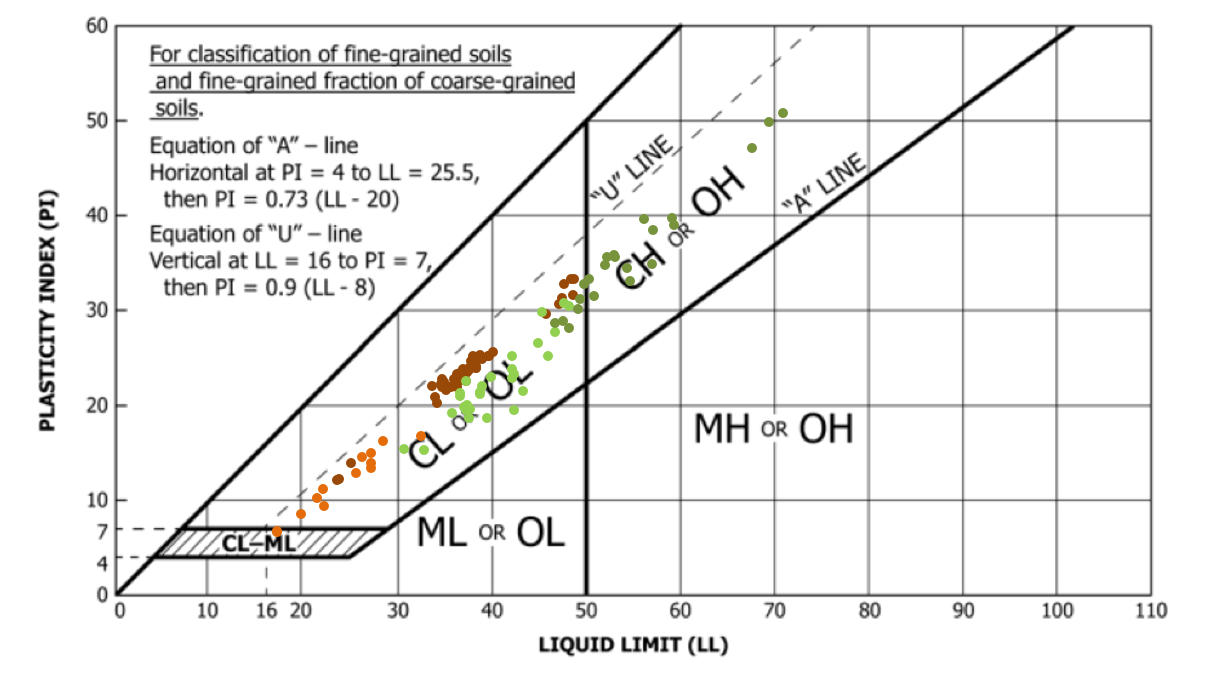
\includegraphics[scale=0.8]{chart-casagrande.png}
    \caption{Диаграмма пластичности Казагранде} \label{Fig:Caz}
  \end{figure}


Для оценки свойств и~определения характерных границ минерального состава на диаграмме Казагранде определены (на основе анализа эмпирических данных) две характерных граничных линии с~уравнениями:

\begin{subequations}
    \label{eq:over}
    \begin{align}
        \label{eq:a}
        \text{А-линия "--- } & PI = 0,73 (LL - 20),
        \\
        \label{eq:u}
        \text{U-линия "--- } & PI = 0,9 (LL - 8).
    \end{align}
\end{subequations}

Можно отметить, что гляциальные и~постгляциальные отложения достаточно много изучались исследователями по всему миру. Так S. Boulton и~M.~Paul  предложили линейное соотношение между  индексом пластичности и~верхним пределом текучести  для грунтов ледникового происхождения, которое получило название <<T-линия>> (Boulton, Paul, 1976) \cite{boulton1976}. Представленное ими линейное уравнение имеет вид:

\begin{equation}
    \label{eq:t}
    \text{T-линия "--- } PI = 0,73 (LL-11).
\end{equation}

Это уравнение лежит между двумя границами <<A-линии>> и~<<U-линии>> на классической диаграмме Казагранде (рис \ref{Fig:Caz}). Представленные результаты лабораторных испытаний пределов Аттенберга показывают, что образцы лежат между <<A и~U-линиями>> близко к~уравнению <<Т-линии>>. Пластичность глинистых разновидностей в~значительной степени зависит не только от содержания глинистых частиц, но и~от минерального состава (Васенин, 2018) \cite{vasenin2018}.

Диаграмма Скемптона \ref{Fig:Skt} была рассмотрена в~1953 году в~его работе для оценки активности грунта \cite{skempton1953}.
Активность грунта "--- показатель, который определяется как отношения индекса пластичности к~массовому содержанию глинистой фракции:

\begin{equation}
    \label{eq:act}
    ACT = \frac{PI}{C_{0,002}}
\end{equation}

\begin{figure}[ht]
    \centering
    \small
    \pgfplotsset{
%samples=15,
width=0.75\linewidth,
xlabel={Содержание глинистой фракции $C_{0.002}$, \%},
ylabel={Индекс пластичности $PI$, \%},
%extra y ticks={45},
legend pos=north west,
legend cell align={left},
}

\begin{tikzpicture}
	\begin{axis}[
	%	grid=major,
	%log plot exponent style/.style={
	%/pgf/number format/fixed,
	%/pgf/number format/use comma,
	%/pgf/number format/precision=2,
	%},
	ymin = 0,
	xmin = 0,
	ymax = 50,
	xmax = 30,
	domain=0:30,
	]
		%\addplot coordinates{(0,0) (30, 50)};
		%node[pos=0.8,above] {$ACT = 1.4$};
		%node[midway,above left] {$d$};
		%node[pos=0.2,below] {$ACT = 0.75$};

		%\addplot [ no marks] {x};

		\addplot[only marks, mark=*, red!70!orange!80!black] table [x=Clay, y=PI, col sep=semicolon] {data/skempton-activity-6.csv};
		\addlegendentry{ИГЭ-6}

		\addplot[only marks, mark=*, lime!40!black] table [x=Clay, y=PI, col sep=semicolon] {data/skempton-activity-7.csv};
		\addlegendentry{ИГЭ-7}

		\addplot[only marks, mark=*, green!50!lime!30!black] table [x=Clay, y=PI, col sep=semicolon] {data/skempton-activity-8.csv};
		\addlegendentry{ИГЭ-8}

		\addplot[only marks, mark=*, red!80!orange!50!black] table [x=Clay, y=PI, col sep=semicolon] {data/skempton-activity-9.csv};
		\addlegendentry{ИГЭ-9}

		
		\addplot [ no marks] {1.4*x} 
		node[pos=0.85, rotate=35] (endofplotsquare) {};
		\node [above, rotate=35] at (endofplotsquare) {$ACT = 1.40$};


		\addplot [ no marks] {0.75*x}
		node[pos=0.80, rotate=20] (endofplotsquare) {};
		\node [below, rotate=20] at (endofplotsquare) {$ACT = 0.75$};



		%\legend{}
	\end{axis}
\end{tikzpicture}

    \caption{Диаграмма активности Скемптона}
    \label{Fig:Skt}
  \end{figure}

Учитывая корреляционные зависимости между минеральным составом и~величиной индекса пластичности $PI$, можно по величине активности определить вероятный минеральный состав. Существует несколько критериев активности минеральных частиц. Наиболее простой"---по величине активности. 
Грунты считаются неактивными при показателе меньше 0,75; нормальной активности "--- от 0,75 до 1,4; повышенной активности "--- больше 1,4 (Васенин, 2018) \cite{vasenin2018}.


%Показатель активности зависит от взаимного соотношения глинистых минералов в~грунте.
Для построения диаграммы пластичности Казагранде и~активности Скемптона, отечественные показатели по классификации ГОСТ 25100-2011 были пересчитаны в~показатели по USCS (ASTM D 2487 и~ISO 14688-2:2004), 
в соответствии с~корреляционными зависимостями, представленными в~формуле Е.1 Приложения Е ГОСТ 25100-2011.


Для исследованных образцов грунта были вычислены показатели активности, которые представлены в~таблице \ref{tab:ak}.

\begin{table}[ht]
    \centering
    %\small
    \caption{Показатели активности грунтов} \label{tab:ak}
    %\renewcommand*{\arraystretch}{1.2} 
    % p{.15\textwidth}
    \begin{tabular}{clcc}
    %\toprule
    %ИГЭ & Активность &  $ACT$ \\
    %\midrule
    ИГЭ-6 \dotfill &  преимущественно нормальная & 0,91--1,36 \\
    ИГЭ-7 \dotfill &  нормальная & 1,01--1,08 \\
    ИГЭ-8 \dotfill &  преимущественно повышенная & 1,20--3,07 \\
    ИГЭ-9 \dotfill &  преимущественно повышенная & 1,16--2,51\\
    %\bottomrule
    \end{tabular}
    %\\ 
\end{table}
    

Эти данные показывают, что активность глинистого несущего матрикса примерно одинаковая. Глинистые минералы исследованных образцов имеют среднюю или немного повышенную активность.
Также в~пользу такого определения основной группы глинистых минералов свидетельствует типичное распределение образцов на диаграмме пластичности Казагранде (рис \ref{Fig:Caz}) (Васенин, 2018) \cite{vasenin2018}.








